\section{Introduction}
\label{sec:introduction}

The paradigm shift driven by foundation models~\citep{bommasani2021opportunities} is revolutionizing the communities who study sequential decision-making problems~\citep{yang2023foundation}, with innovations focusing on control~\citep{ahn2022saycan,liang2022code,jiang2022vima,brohan2022rt1}, planning~\citep{wang2023voyager,huang2022language,huang2022inner,wang2023describe,driess2023palme}, pre-trained visual representation~\citep{nair2022r3m,ma2022vip,radosavovic2022realworld,majumdar2023search}, among others.
Despite the progress, the data-hungry nature makes the application of Transformer~\citep{vaswani2017attention} agents extremely challenging in data-scarce domains like robotics~\citep{mandlekar2018roboturk,mandlekar2021matters,ebert2021bridge,jiang2022vima,brohan2022rt1}.
This leads us to the question: Can we maximize the utilization of limited data, regardless of their optimality and construction, to foster more efficient learning?

To this end, this paper introduces a novel algorithm named \textit{Cross-Episodic Curriculum} (\cec), a method that explicitly harnesses the shifting distributions of multiple experiences when organized into a curriculum.
The key insight is that sequential \textit{cross-episodic} data manifest useful learning signals that do not easily appear in any separated training episodes.\footnote{Following the canonical definition in \citet{sutton2018reinforcement}, we refer to the sequences of agent-environment interaction with clearly identified initial and terminal states as ``episodes''. We interchangeably use ``episode'', ``trial'', and ``trajectory'' in this work.}
As illustrated in Figure~\ref{fig:pull_fig}, \cec realizes this through two stages: 1) formulating curricular sequences to capture (a) the policy improvement on single environments, (b) the learning progress on a series of progressively harder environments, or (c) the increase of demonstrators' proficiency; 
and 2) causally distilling policy improvements into the model weights of Transformer agents through \emph{cross-episodic attention}.
When a policy is trained to predict actions at current time steps, it can trace back beyond ongoing trials and internalize improved behaviors encoded in curricular data, thereby achieving efficient learning and robust deployment when probed with visual or dynamics perturbations.
Contrary to prior works like Algorithm Distillation (AD, \citet{laskin2023incontext}) which, at test time, samples and retains a single task configuration across episodes for in-context refinement, our method, \cec, prioritizes zero-shot generalization across a distribution of test configurations. With \cec, agents are evaluated on a new task configuration in each episode, emphasizing adaptability to diverse tasks.

\begin{figure}[!t]
    \centering
    \vspace{-0.1in}
    \makebox[\textwidth][c]{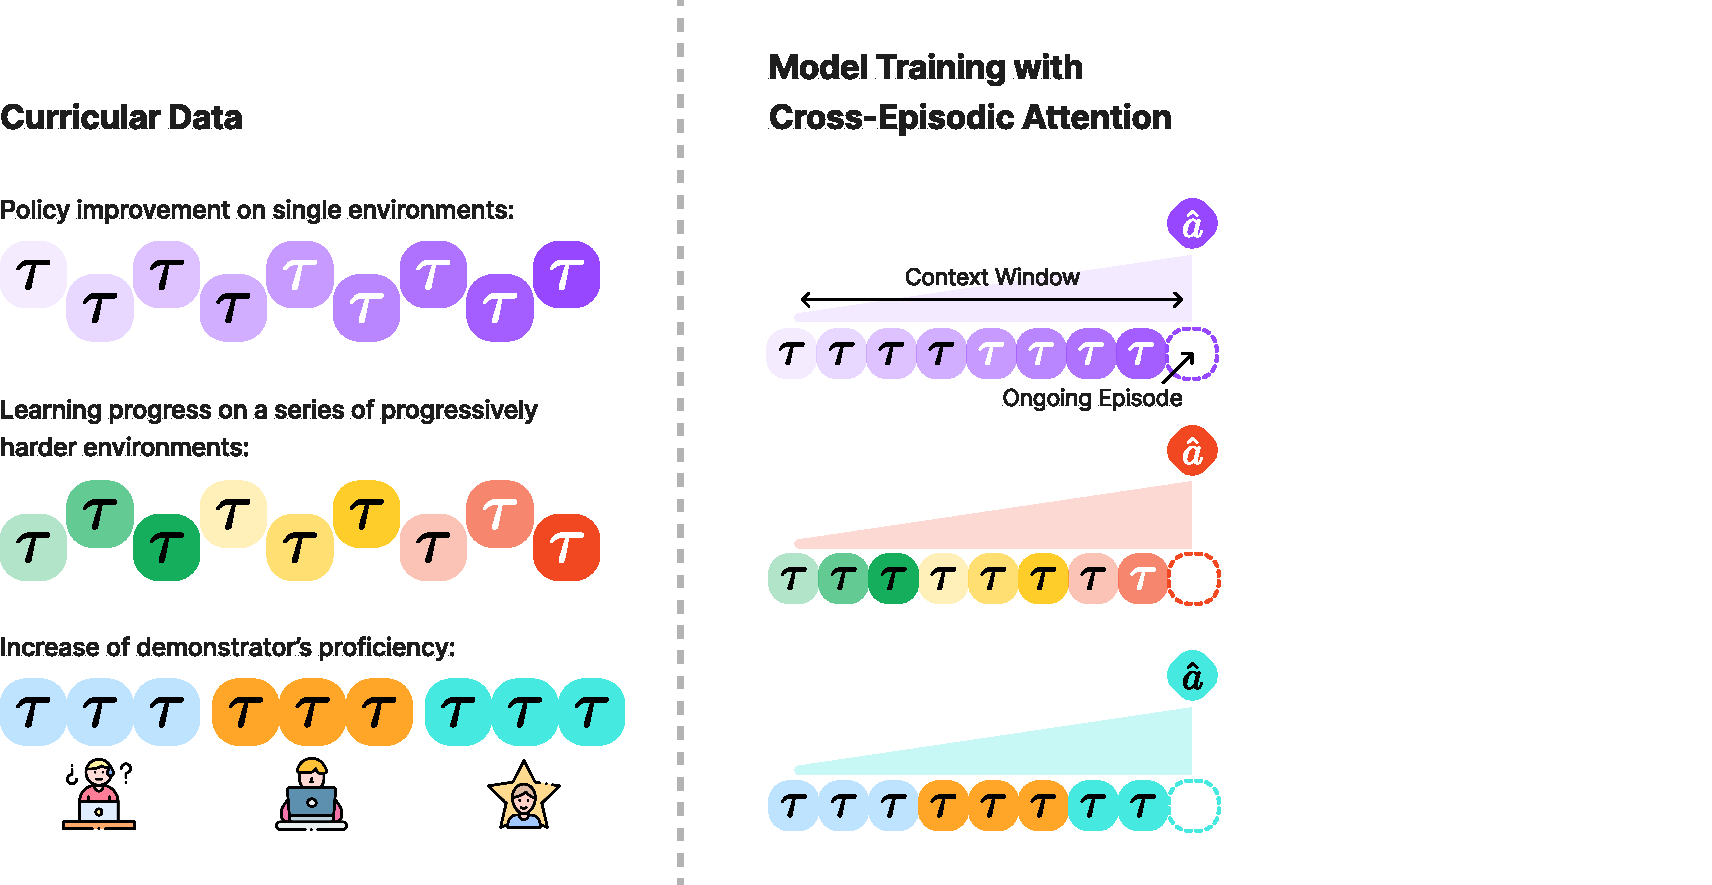
\includegraphics[width=0.9\textwidth]{fig/pull_fig-fig.pdf}}
    \caption{\textbf{Cross-episodic curriculum for Transformer agents.}
    \cec involves two major steps:
    \textit{\mbox{1) Preparation of curricular data.}} We order multiple experiences such that they explicitly capture curricular patterns. For instance, they can be policy improvement in single environments, learning progress in a series of progressively harder environments, or the increase of the demonstrator's expertise.
    \textit{2) Model training with cross-episodic attention.} When training the model to predict actions, it can trace back beyond the current episode and internalize the policy refinement
    for more efficient learning.
    Here each $\tau$ represents an episode (trajectory). $\hat{a}$ refers to actions predicted by the model.
    Colored triangles denote causal Transformer models.
    }
    \label{fig:pull_fig}  
\end{figure}




We investigate the effectiveness of \cec in enhancing sample efficiency and generalization with two representative case studies.
They are: 1) Reinforcement Learning (RL) on DeepMind Lab~(DMLab)~\citep{beattie2016deepmind}, a 3D simulation encompassing visually diverse worlds, complicated environment dynamics, ego-centric pixel inputs, and joystick control; and 2) Imitation Learning (IL) from mixed-quality human demonstrations on RoboMimic~\citep{mandlekar2021matters}, a framework designed to study robotic manipulation with proprioceptive and external camera observations and continuous control.
Despite RL episodes being characterized by state-action-reward tuples and IL trajectories by state-action pairs, our method exclusively employs state-action pairs in its approach.

In challenging embodied navigation tasks, despite significant generalization gaps (Table~\ref{table:dmlab_exp_setting}),
our method surpasses concurrent and competitive method Agentic Transformer (AT, \citet{liu2023emergent}).
It also significantly outperforms popular offline RL methods such as Decision Transformer (DT, \citet{chen2021decisiontransformer}) and baselines trained on expert data, with the same amount of parameters, architecture, and data size.
It even exceeds RL oracles directly trained on test task distributions 
by $50\%$ in a \emph{zero-shot} manner. 
\cec also yields robust embodied policies that are up to $1.6\times$ better than RL oracles when zero-shot probed with unseen environment dynamics.
When learning continuous robotic control, \cec successfully solves two simulated manipulation tasks, matching and outperforming previous well-established baselines~\cite {mandlekar2021matters,fujimoto2018offpolicy,kumar2020conservative}.
Further ablation reveals that \cec with cross-episodic attention is a generally effective recipe for learning Transformer agents, especially in applications where sequential data exhibit moderate and smooth progression.



























